\section{ЦЕЛЬ И ЗАДАЧИ РАБОТЫ} %поменять с программами местами

Численное моделирование течения струй газа с неравновесными химическими процессами представляет собой сложную многопараметрическую задачу, требующую комплексного подхода к описанию как гидродинамики потока, так и кинетики химических реакций. Актуальность данной темы обусловлена её практическим значением для аэрокосмической индустрии, энергетики, двигателестроения и других областей, где важны точные прогнозы характеристик газодинамических и химических процессов.

\subsection{Цель работы}

Основной целью данной работы является разработка численной модели и программного обеспечения для расчёта течения реактивных струй газа с учётом неравновесной химической кинетики, а также верификация модели на основе сравнения с экспериментальными данными.

%Конкретные аспекты, на которые направлено исследование, представленные на рисунке \ref{fig:goals}:
Конкретные аспекты, на которые направлено исследование:

\begin{itemize}
    \item моделирование ламинарных и турбулентных течений с химическими реакциями;
    \item учёт неравновесных процессов (диссоциация, рекомбинация, горение);
    \item обеспечение приемлемой точности расчётов при разумных вычислительных затратах;
    \item проверка адекватности модели путём сопоставления с известными экспериментальными и численными данными.
\end{itemize}

Отдельно можно выделить цель сравнения работы полной системы уравнений Навье-Стокса и их параболизованной версии по точности и вычислительным затратам.

%\begin{figure}
%    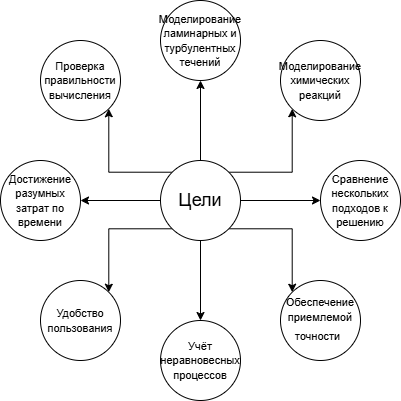
\includegraphics[width=15cm]{2-01-goals}
%    \caption{Основные цели проекта}
%    \label{fig:goals}
%\end{figure}

\subsection{Задачи проекта}

Для достижения поставленной цели в работе решаются следующие задачи (Рис. \ref{fig:tasks}):

\begin{enumerate}
    \item Анализ существующих математических моделей:
    \begin{enumerate}
        \item Обзор уравнений Навье–Стокса и их модификаций для описания течений с химическими реакциями;
        \item Изучение моделей турбулентности ($k-\epsilon$, $SST$ и т.д.), применимых для расчёта реактивных струй;
        \item Анализ кинетических схем для описания неравновесных химических процессов;
    \end{enumerate}
    \item Разработка численного алгоритма:
    \begin{enumerate}
        \item Построение дискретной схемы для решения системы уравнений газовой динамики с химическими источниками;
        \item Реализация методов расчёта турбулентного перемешивания и химических реакций;
        \item Оптимизация вычислительных процедур для снижения ресурсоёмкости;
    \end{enumerate}
    \item Создание программного обеспечения:
    \begin{enumerate}
        \item Разработка программы на основе выбранных математических моделей;
        \item Обеспечение возможности моделирования как ламинарных, так и турбулентных режимов течения;
        \item Реализация визуализации результатов (поля скорости, температуры, концентрации компонент);
        \item Разработка графического пользовательского интерфейса для удобной работы с данными;
    \end{enumerate}
    \item Верификация и валидация модели:
    \begin{enumerate}
        \item Проведение тестовых расчётов для стандартных конфигураций (например, ламинарное и турбулентное истечение струи);
        \item Сравнение численных результатов с экспериментальными данными и решениями других авторов;
        \item Оценка точности и устойчивости разработанного алгоритма;
    \end{enumerate}
    \item Анализ результатов и выводы:
    \begin{enumerate}
        \item Исследование влияния различных факторов (скорость истечения, состав смеси, температура) на структуру течения;
        \item Определение границ применимости модели;
        \item Формулировка рекомендаций для дальнейшего развития.
    \end{enumerate}
\end{enumerate}

\begin{figure}
    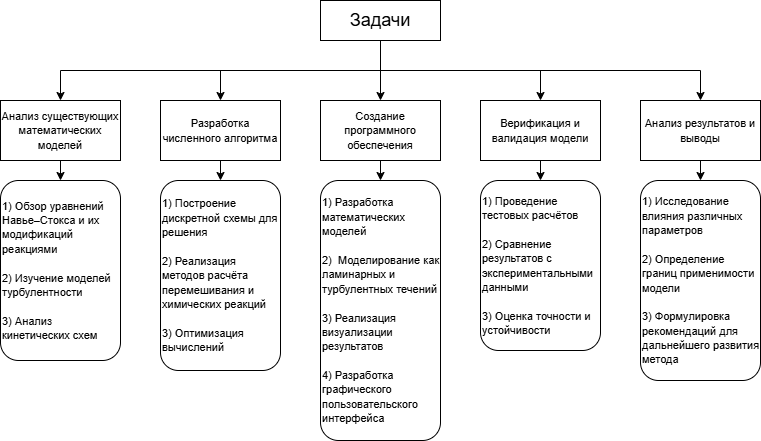
\includegraphics[width=15cm]{2-01-tasks}
    \caption{Задачи проекта}
    \label{fig:tasks}
\end{figure}

При выполнении работы были использованы лишь некоторые модели турбулентности, однако существует возможность добавления и таких моделей, как $k-\epsilon$ или $SST$ при дальнейшем развитии.

\subsection{Научная новизна и практическая значимость работы}

Научная новизна исследования заключается в следующем:

\begin{itemize}
    \item разработана комплексная модель, сочетающая методы расчёта турбулентных течений и неравновесной химической кинетики;
    \item реализована гибкая система визуализации многопараметрических данных;
    \item предложены оптимизированные алгоритмы, позволяющие проводить расчёты с приемлемой точностью без чрезмерных вычислительных затрат;
    \item проведена верификация модели на широком наборе тестовых случаев, включая высокоскоростные и химически реагирующие течения;
    \item установлены критерии применимости параболизированной модели для течений с химическими реакциями;
    \item выявлена зависимость погрешности расчёта от степени детализации химического механизма;
    \item проведено сравнение точности параболизованной системы уравнений и полного Навье-Стокса на широком наборе тестовых случаев.
\end{itemize}

Результаты работы, при дальнейшем развитии, могут быть использованы:

\begin{itemize}
    \item при проектировании реактивных двигателей и сопловых аппаратов;
    \item в задачах моделирования горения и смесеобразования в энергетических установках;
    \item в научных исследованиях, связанных с неравновесными газодинамическими процессами.
\end{itemize}

Перспективы дальнейшего развития:

\begin{itemize}
\item расширение модели на многофазные течения;
\item интеграция с методами машинного обучения;
\item разработка облачной версии вычислительного комплекса.
\end{itemize}

Таким образом, данная работа направлена на создание инструмента для численного моделирования сложных газодинамических процессов, что позволит улучшить понимание физики течений с химическими реакциями и оптимизировать инженерные расчёты.
